% presentation
%\documentclass[compress,draft]{beamer}
\documentclass[compress,aspectratio=1610,fleqn]{beamer}
%\documentclass[compress,aspectratio=1610,handout]{beamer}
\usepackage{../mtex,fancyvrb,booktabs,multirow,makecell}
\usepackage{tikz,pgfplots,multicol,bbding}
\usetikzlibrary{shapes,calc,angles,quotes,external}
\usepackage{tasks}
\settasks{counter-format=tsk[a]),label-width=1em,before-skip=0.5em}
\RenewTasks{enumerate}[\item]

\makeatletter
\newcommand*{\overlaynumber}{\number\beamer@slideinframe}
\tikzset{
  beamer externalizing/.style={%
    execute at end picture={%
      \tikzifexternalizing{%
        \ifbeamer@anotherslide
        \pgfexternalstorecommand{\string\global\string\beamer@anotherslidetrue}%
        \fi
      }{}%
    }%
  },
  external/optimize=false
}
\let\orig@tikzsetnextfilename=\tikzsetnextfilename
\renewcommand\tikzsetnextfilename[1]{\orig@tikzsetnextfilename{#1-\overlaynumber}}

\DeclareMathOperator*{\argmin}{argmin}
\makeatother

\tikzset{every picture/.style={beamer externalizing}}
\tikzexternalize[prefix=tikz/]

\newcommand{\rz}{\ensuremath \mathbb{R}}   %reelle Zahlen


%\usepackage{subfigure}
\usepackage[labelformat=empty]{subcaption}
\captionsetup{compatibility=false}
%\usepackage[inline]{enumitem}
\newcommand\paraitem{%
  \;
  \makebox[\labelwidth][r]{%
    \makelabel{%
      \usebeamertemplate{itemize \beameritemnestingprefix item}}}\hskip\labelsep}


\newcommand{\SO}{\mathrm{SO}(3)}
\newcommand{\rot}[1]{\mathbf{#1}}
\newcommand{\ds}{\displaystyle}
\newcommand{\R}{\mathbb R}
\renewcommand{\S}{\mathbb S}
\newcommand{\conj}[1]{\overline{#1}}
\newcommand{\norm}[1]{\lVert #1\rVert}
\newcommand{\abs}[1]{\lvert #1\rvert}
\newcommand{\laplace}{\triangle}

\DeclareMathOperator{\argmax}{argmax}


\newcommand{\mytriangle}[1]{\tikz{\node[draw=#1,fill=#1,isosceles
triangle,isosceles triangle stretches,shape border rotate=90,minimum
width=0.2cm,minimum height=0.2cm,inner sep=0pt] at (0,0) {};}}

\usetikzlibrary{fit}
% \tikzset{%
%   highlight/.style={rectangle,rounded corners,fill=red!15,draw,
%     fill opacity=0.5,thick,inner sep=0pt}
%   }
\tikzset{%
  highlight/.style={rectangle,rounded corners,draw,red,
    fill opacity=0.5,thick,inner sep=0pt}
}
% see https://tex.stackexchange.com/questions/40028/highlight-elements-in-the-matrix

\newcommand{\tikzmark}[2]{\tikz[overlay,remember picture,
  baseline=(#1.base)] \node (#1) {#2};}
%
\newcommand{\Highlight}[1][submatrix]{%
    \tikz[overlay,remember picture]{
    \node[highlight,fit=(left.north west) (right.south east)] (#1) {};}
}


\renewcommand{\arraystretch}{1.4}

\author{Ralf Hielscher}

\title{Density Functions}

\institute{Faculty of Mathematics and Informatics,\\
	TU Bergakademie Freiberg, Germany}

\date{MTEX Workshop 2024}


\begin{document}

\begin{frame}
  \maketitle{}
\end{frame}


\begin{frame}[fragile]
  \frametitle{From Points to Density Functions}


  \begin{columns}

    \begin{column}{0.6\textwidth}
      \begin{lstlisting}[style=input]
h = Miller(1,0,-1,1,cs)
plotPDF(ori,h,'all','layout',[2 1])
\end{lstlisting}

\pause

      \begin{lstlisting}[style=input]
plotPDF(ori,h,'MarkerAlpha',0.1)
\end{lstlisting}

\pause

      \begin{lstlisting}[style=input]
plot(ori,h,'contour')
\end{lstlisting}

\pause

      \begin{lstlisting}[style=input]
plotPDF(ori,h,'pcolor')
\end{lstlisting}

\medskip
\pause

You can do the same with
\begin{itemize}
\item axes
\item orientations
\item misorientations
\end{itemize}

\medskip
\pause

\structure{But, how does it work?}

    \end{column}

    \begin{column}{0.24\textwidth}
      \vspace{-0.5cm}
      \only<1>{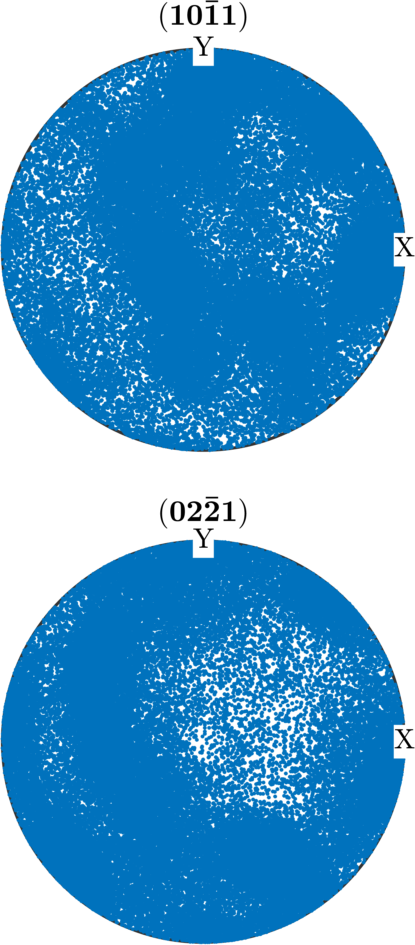
\includegraphics[width=\textwidth]{pic/scatterV}}
      \only<2>{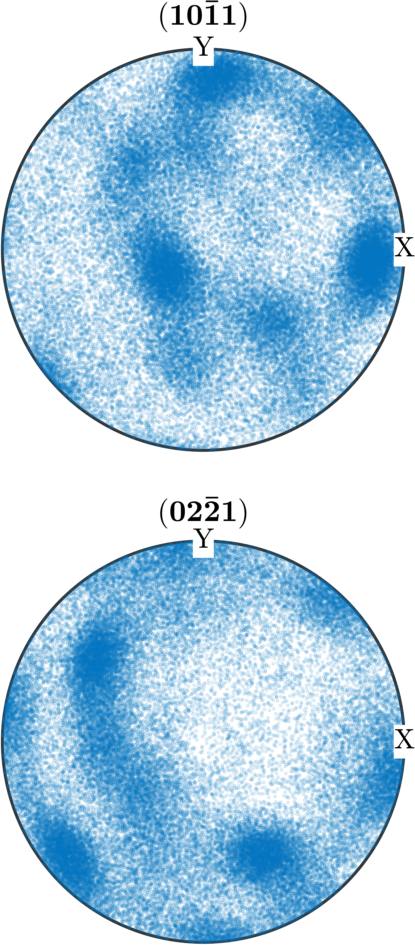
\includegraphics[width=\textwidth]{pic/alphaV}}
      \only<3>{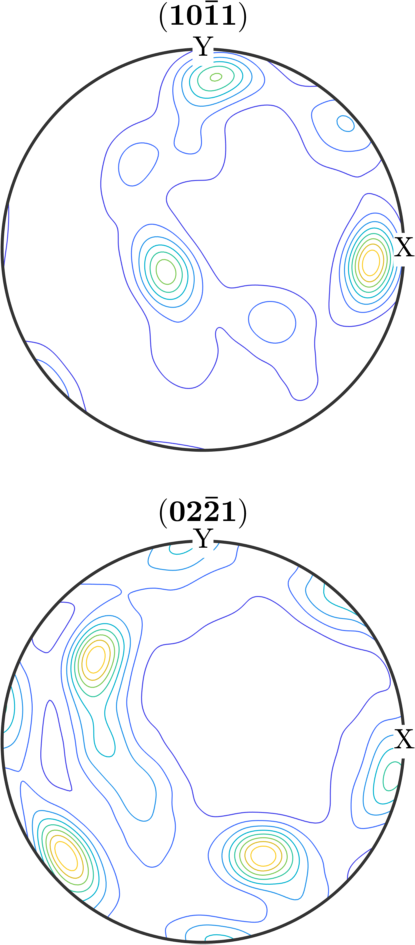
\includegraphics[width=\textwidth]{pic/contourV}}
      \only<4->{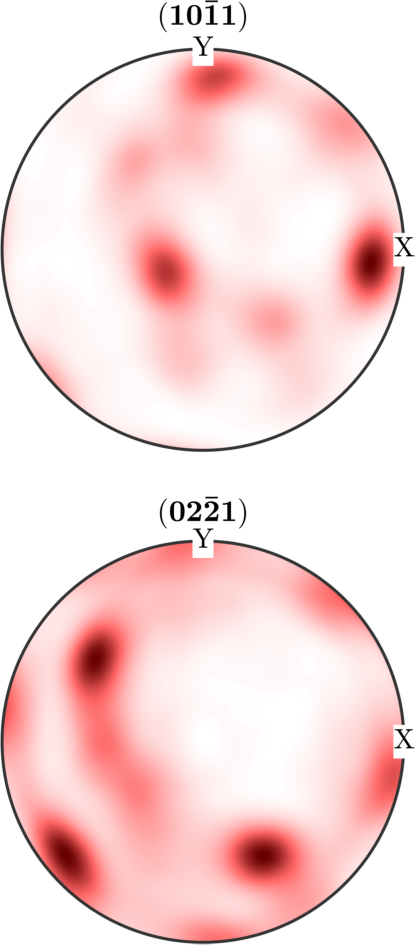
\includegraphics[width=\textwidth]{pic/pcolorV}}

    \end{column}

  \end{columns}

\end{frame}


\begin{frame}
  \frametitle{Kernel Density Estimation}

  \medskip
  
  \structure{Input:} some random numbers ${\color{red!90!black}x_{1},\ldots,x_{N}}$

  \medskip
  
  \uncover<2->{\structure{Assumption:} there is an underlying probability density function
    ${\bf \color{green!60!black}f} \colon \rz \to \rz_{+}$}

  \medskip
  
  \uncover<3->{\structure{Goal}: Find an approximation ${\bf \color{blue}f^{*}}$ of ${\bf \color{green!60!black}f}$}

  \bigskip

  \begin{overlayarea}{\textwidth}{9cm}
    \center
    \begin{onlyenv}<1-7|handout:0>
      \begin{tikzpicture}
        \begin{axis}[xtick=-1, ytick=-1,smooth,width=\textwidth, height=7cm, ymin=0,ymax=7,xmin=0,xmax=1,enlargelimits=false]
          % the true density
          \only<2->{\addplot[mark=none,very thick,green!60!black] table[x index=0,y index=1]
          {matlab/example.txt};}
          % the random sample
          \only<1,2,3,4,5,6,7>{\addplot[mark=o, only marks, red!90!black, thick] table[x index=0,y index=1]
          {matlab/sample_1.txt};}
          % the histogram
          \only<4>{\addplot[ybar interval, fill=blue!30!white] table[x index=0,y index=1]
          {matlab/hist.txt};}
          % the kernel
          \only<5>{\addplot[mark=none,blue, thick] table[x index=0,y index=22]
          {matlab/example.txt};}
          % the kernel density estimator
          \only<6>{
            \foreach \x in {4,5,6,...,22}
            \addplot[mark=none,blue] table[x index=0,y index=\x]
            {matlab/example.txt};
          }
          \only<7>{\addplot[mark=none,blue,very thick] table[x index=0,y index=2]
            {matlab/example.txt};}
          % \only<5>{
%             \addplot[mark=o, only marks, red] table[x index=0,y index=1]
%             {matlab/sample_2.txt};
%             \addplot[mark=none,blue,very thick] table[x index=0,y index=3]
%             {matlab/example.txt};
%           }

        \end{axis}
      \end{tikzpicture}
    \end{onlyenv}

    \only<8->{
      \begin{block}{Kernel Density Estimator}
        kernel function $\psi \colon \rz \to \rz$, $\int_{\rz} \psi(x)
        dx = 1$
        \begin{equation*}
          f^*_{N,\psi}(x) = \frac{1}{N} \sum_{n = 1}^N \psi(x-X_{n}),
        \end{equation*}
      \end{block}
    }


    \begin{itemize}
    \item<9-> The idea generalizes to arbitrary data, i.e., for specimen
      directions, axes, crystal directions, orientations, misorientations.
    \item<10-> The estimated function $f^*_{N,\psi}$ heavily depends on the
      kernel function $\psi$.

    \end{itemize}
  \end{overlayarea}
\end{frame}





\begin{frame}
  \frametitle{Specific Density Functions}


  \begin{definition}[Orientation Density Function]
  \begin{equation*}
    \mathtt{odf}(g) = \frac{1}{V} \frac{dV(g)}{\mathrm dg}
  \end{equation*}
  \end{definition}

  \begin{table}
    \centering
    \begin{tabular}{lll}
      objects
      & description
      & density function \\
      \midrule
      $\mathtt{ori}$
      & orientations
      & orientation density function (ODF) \\
      $\mathtt{ori} * \{hkl\}$
      & pole figure directions
      & pole density function (PDF) \\
      $\mathtt{ori}^{-1} * xyz$
      & inverse pole figure directions
      & inverse pole density function (IPDF)\\
      $\mathtt{ori_{1}}^{-1}*\mathtt{ori_{2}}$
      & misorientations
      & misorientation density function (MDF)\\
      $\omega$
      & misorientation angles
      & misorientation angle distribution function \\
      $\vec \eta$
      & misorientation axes
      & misorientation axes distribution function
    \end{tabular}
  \end{table}

\end{frame}


\begin{frame}[fragile]
  \frametitle{Density Estimation in MTEX}

  \begin{overlayarea}{\textwidth}{0.85\textheight}
  orientation distribution function
  \vspace{-0.2cm}
\begin{lstlisting}[style=input]
ori = ebsd('phaseName').orientations;
odf = calcDensity(ori)
\end{lstlisting}
\begin{onlyenv}<1>
  \vspace{-0.2cm}
  \begin{lstlisting}[style=output]
odf = /+SO3FunHarmonic+/ (/+Quartz+/ -> xyz)
  isReal: true
  bandwidth: 25
  weight: 1
  \end{lstlisting}
\end{onlyenv}
\begin{onlyenv}<2->
pole density function  \vspace{-0.2cm}
\begin{lstlisting}[style=input]
h = Miller(1,0,0,ori.CS);
pdf = calcDensity(ori.symmetrise * h)
\end{lstlisting}
\end{onlyenv}
\begin{onlyenv}<2>
  \vspace{-0.2cm}
  \begin{lstlisting}[style=output]
pdf = /+S2FunHarmonic+/
 bandwidth: 25
  \end{lstlisting}
\end{onlyenv}

\begin{onlyenv}<3->
inverse pole density function
\vspace{-0.2cm}
\begin{lstlisting}[style=input]
r = vector3d.Z;
ipdf = calcDensity(inv(ori.symmetrise) * r)
\end{lstlisting}
\end{onlyenv}
\begin{onlyenv}<3>
  \vspace{-0.2cm}
  \begin{lstlisting}[style=output]
ipdf = /+S2FunHarmonicSym+/ (/+Quartz+/)
 bandwidth: 25
\end{lstlisting}
\end{onlyenv}

\begin{onlyenv}<4->
boundary misorientation density function\vspace{-0.2cm}
\begin{lstlisting}[style=input]
mori = grains.boundary('phase1','phase2').misorientation
mdf = calcDensity(mori)
\end{lstlisting}
\end{onlyenv}
\end{overlayarea}
\end{frame}

\begin{frame}[fragile]
  \frametitle{Operation with Functions}
  \begin{columns}
    \begin{column}{0.6\textwidth}
      \vspace{-0.5cm}
      \begin{overlayarea}{\textwidth}{0.85\textheight}
\begin{lstlisting}[style=input]
plot(ipdf)
\end{lstlisting}
\pause
\vspace{-0.3cm}
\begin{lstlisting}[style=input]
contour, contourf, plot3d, plotSection
\end{lstlisting}

\pause
\vspace{0.1cm}

function value at a point \vspace{-0.2cm}
\begin{lstlisting}[style=input]
ipdf.eval(Miller(1,0,0,cs))
\end{lstlisting}

\pause
\vspace{0.1cm}

arbitrary mathematical operations
\vspace{-0.2cm}
\begin{lstlisting}[style=input]
f1 + f2, f1 .* f2
\end{lstlisting}

\pause
\vspace{0.1cm}

rotate
\vspace{-0.2cm}
\begin{lstlisting}[style=input]
rotate(pdf,rot)
\end{lstlisting}

\pause
\vspace{0.1cm}

min / max
\vspace{-0.2cm}
\begin{lstlisting}[style=input]
[val, pos] = max(ipdf,'numLocal',2)
\end{lstlisting}

\pause
\vspace{0.1cm}

average
\vspace{-0.2cm}
\begin{lstlisting}[style=input]
sum(pdf), mean(pdf),
\end{lstlisting}

\end{overlayarea}

\end{column}
\begin{column}{0.35\textwidth}
  \centering
  \only<1>{
    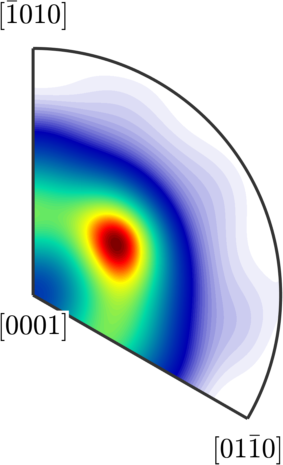
\includegraphics[width=0.8\textwidth]{pic/ipdf}}
  \only<2>{
    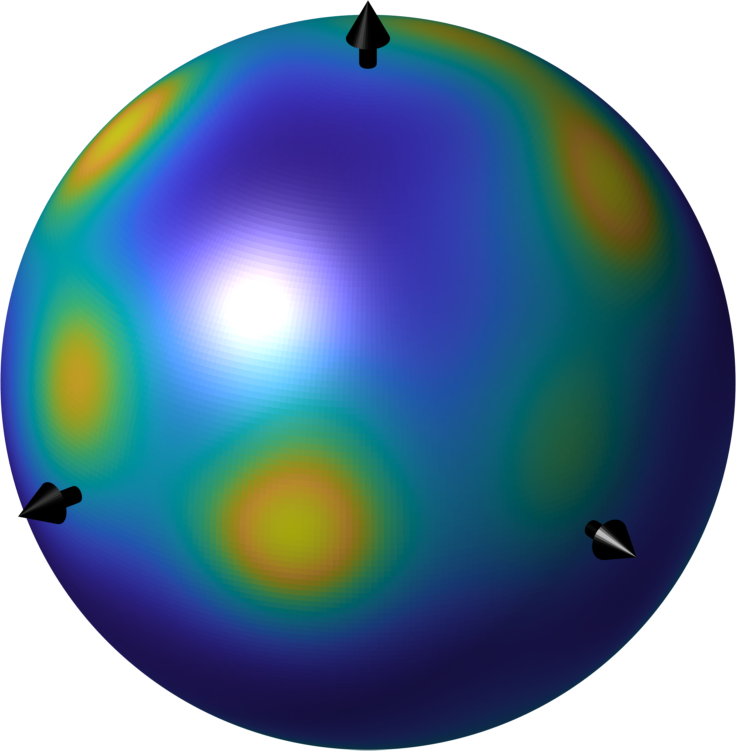
\includegraphics[width=\textwidth]{pic/pdf3d}}
\end{column}
  \end{columns}

\end{frame}

\begin{frame}[fragile]
  \frametitle{The Influence of the Halfwidth}

  \begin{columns}
    \begin{column}{0.72\textwidth}

      \begin{lstlisting}[style=input]
odf = calcDensity(ori,'halfwidth',2.5*degree)
\end{lstlisting}
\pause
\vspace{-0.2cm}
\begin{lstlisting}[style=input]
odf = calcDensity(ori,'halfwidth',5*degree)
\end{lstlisting}
\pause
\vspace{-0.2cm}
\begin{lstlisting}[style=input]
odf = calcDensity(ori,'halfwidth',7.5*degree)
\end{lstlisting}
\pause
\vspace{-0.2cm}
\begin{lstlisting}[style=input]
odf = calcDensity(ori,'halfwidth',10*degree)
\end{lstlisting}
\pause
\vspace{-0.2cm}
\begin{lstlisting}[style=input]
odf = calcDensity(ori,'halfwidth',15*degree)
\end{lstlisting}
\pause

\begin{lstlisting}[style=input]
psi = calcKernel(ori)
odf = calcDensity(ori,'kernel',psi)
\end{lstlisting}

      \begin{itemize}
      \item There is no one to one relationship between a discrete sampling
        and the density function.
      \item The critical parameter is the halfwidth of the kernel function.
      \item Many properties of the estimated ODF depend also heavily on the
        halfwidth.
      \end{itemize}


    \end{column}
    \begin{column}{0.23\textwidth}
      \centering
      \only<1>{
\includegraphics[width=\textwidth]{pic/pdf25}}
      \only<2>{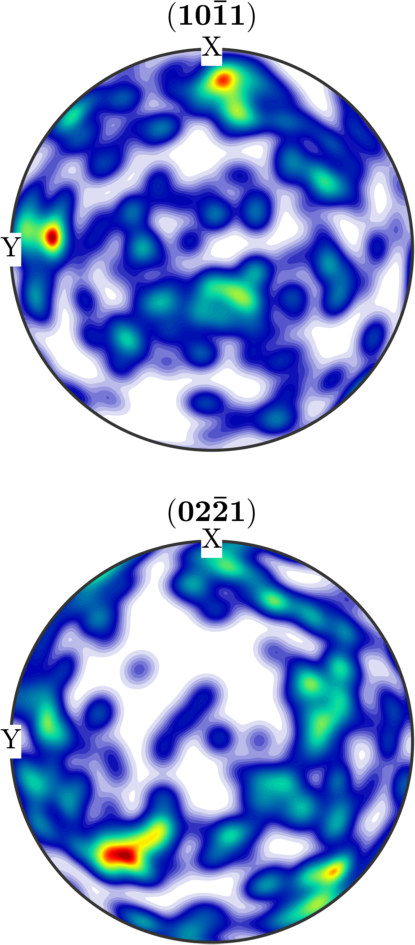
\includegraphics[width=\textwidth]{pic/pdf5}}
      \only<3>{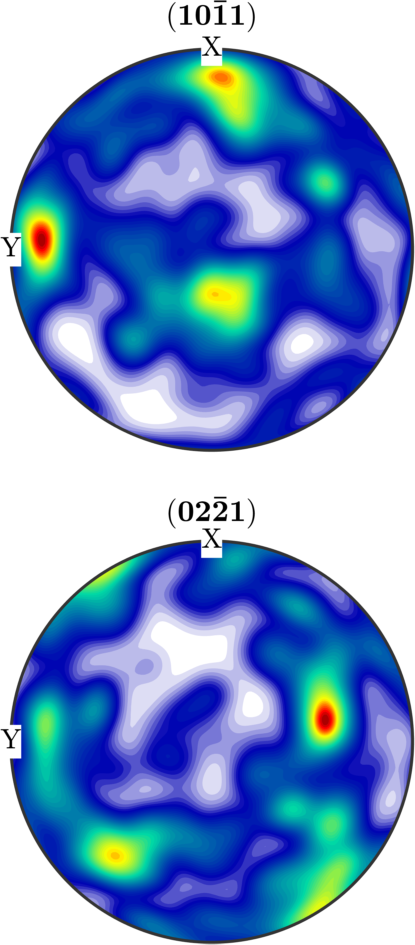
\includegraphics[width=\textwidth]{pic/pdf75}}
      \only<4>{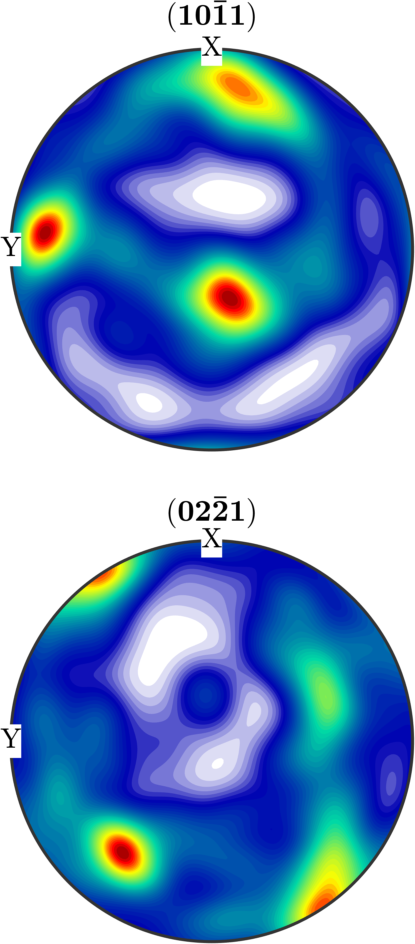
\includegraphics[width=\textwidth]{pic/pdf10}}
      \only<5>{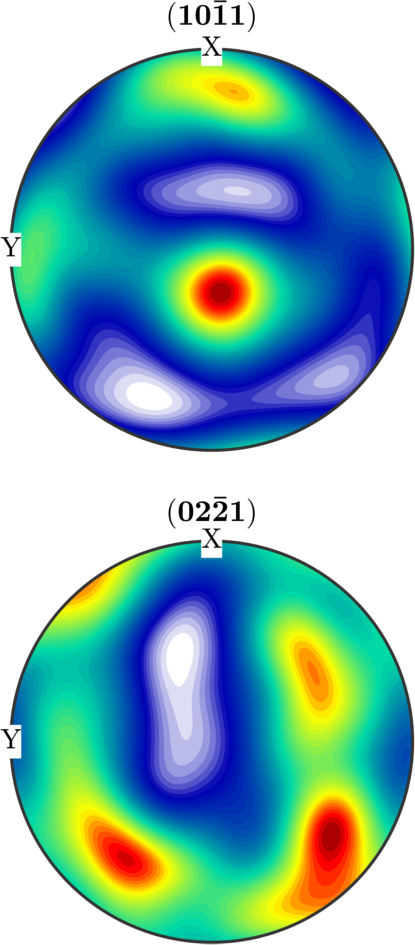
\includegraphics[width=\textwidth]{pic/pdf15}}
      \only<6>{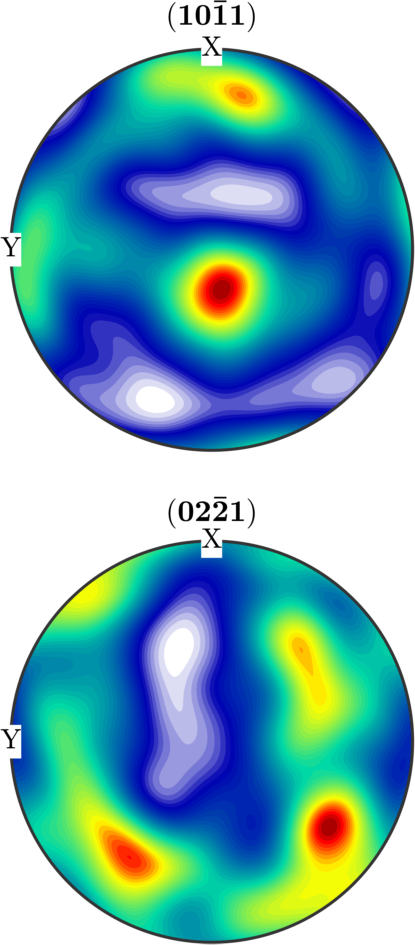
\includegraphics[width=\textwidth]{pic/pdfPsi}}

\end{column}
  \end{columns}



\end{frame}


\begin{frame}[fragile]
  \frametitle{The Inverse Problem}

  Given a density function we may also ask for a corresponding random
  sampling.

  \pause
  \medskip

  orientations randomly sampled from an ODF \vspace{-0.2cm}
  \begin{lstlisting}[style=input]
ori = odf.discreteSample(1000)
  \end{lstlisting}

  \pause
  \medskip

  pole figure directions randomly sampled from an PDF \vspace{-0.2cm}
  \begin{lstlisting}[style=input]
r = pdf.discreteSample(1000)
  \end{lstlisting}

  \pause
  \medskip

  Random samplings are important for crystal plasticity simulations,
  e.g. Taylor, ALAMEL, VPSC.
  \vspace{-0.2cm}
  \begin{lstlisting}[style=input]
export_VPSC(odf,'file.txt','points',10000)
  \end{lstlisting}

  \medskip
  \pause

  An alternative approach for representing ODFs is intensity values at a grid
  of orientations.
  \vspace{-0.2cm}
  \begin{lstlisting}
ori = equispacedSO3Grid(cs,'points',10000)
ori = regularSO3Grid(cs,'resulution',5*degree)
val = odf.eval(ori)
  \end{lstlisting}

\end{frame}

\begin{frame}[fragile]
  \frametitle{Model ODFs}

  \begin{columns}
    \begin{column}{0.5\textwidth}

  \begin{lstlisting}[style=input]
cs = crystalSymmetry('432')
ss = specimenSymmetry('222')

ori1 = orientation.brass(cs,ss)
ori2 = orientation.goss(cs,ss)

odf = 0.2 * uniformODF(cs) ...
  + 0.4 * unimodalODF(ori1, ...
     'halfwidth',10*degree) ...
  + 0.4 * unimodalODF(ori2, ...
     'halfwidth',20*degree)
\end{lstlisting}

\pause
\medskip

  \begin{lstlisting}[style=input]
f = fibre.beta(cs,ss)
odf = fibreODF(f,...
    'halfwidth',5*degree)
  \end{lstlisting}
\end{column}
\begin{column}{0.45\textwidth}
  \only<1>{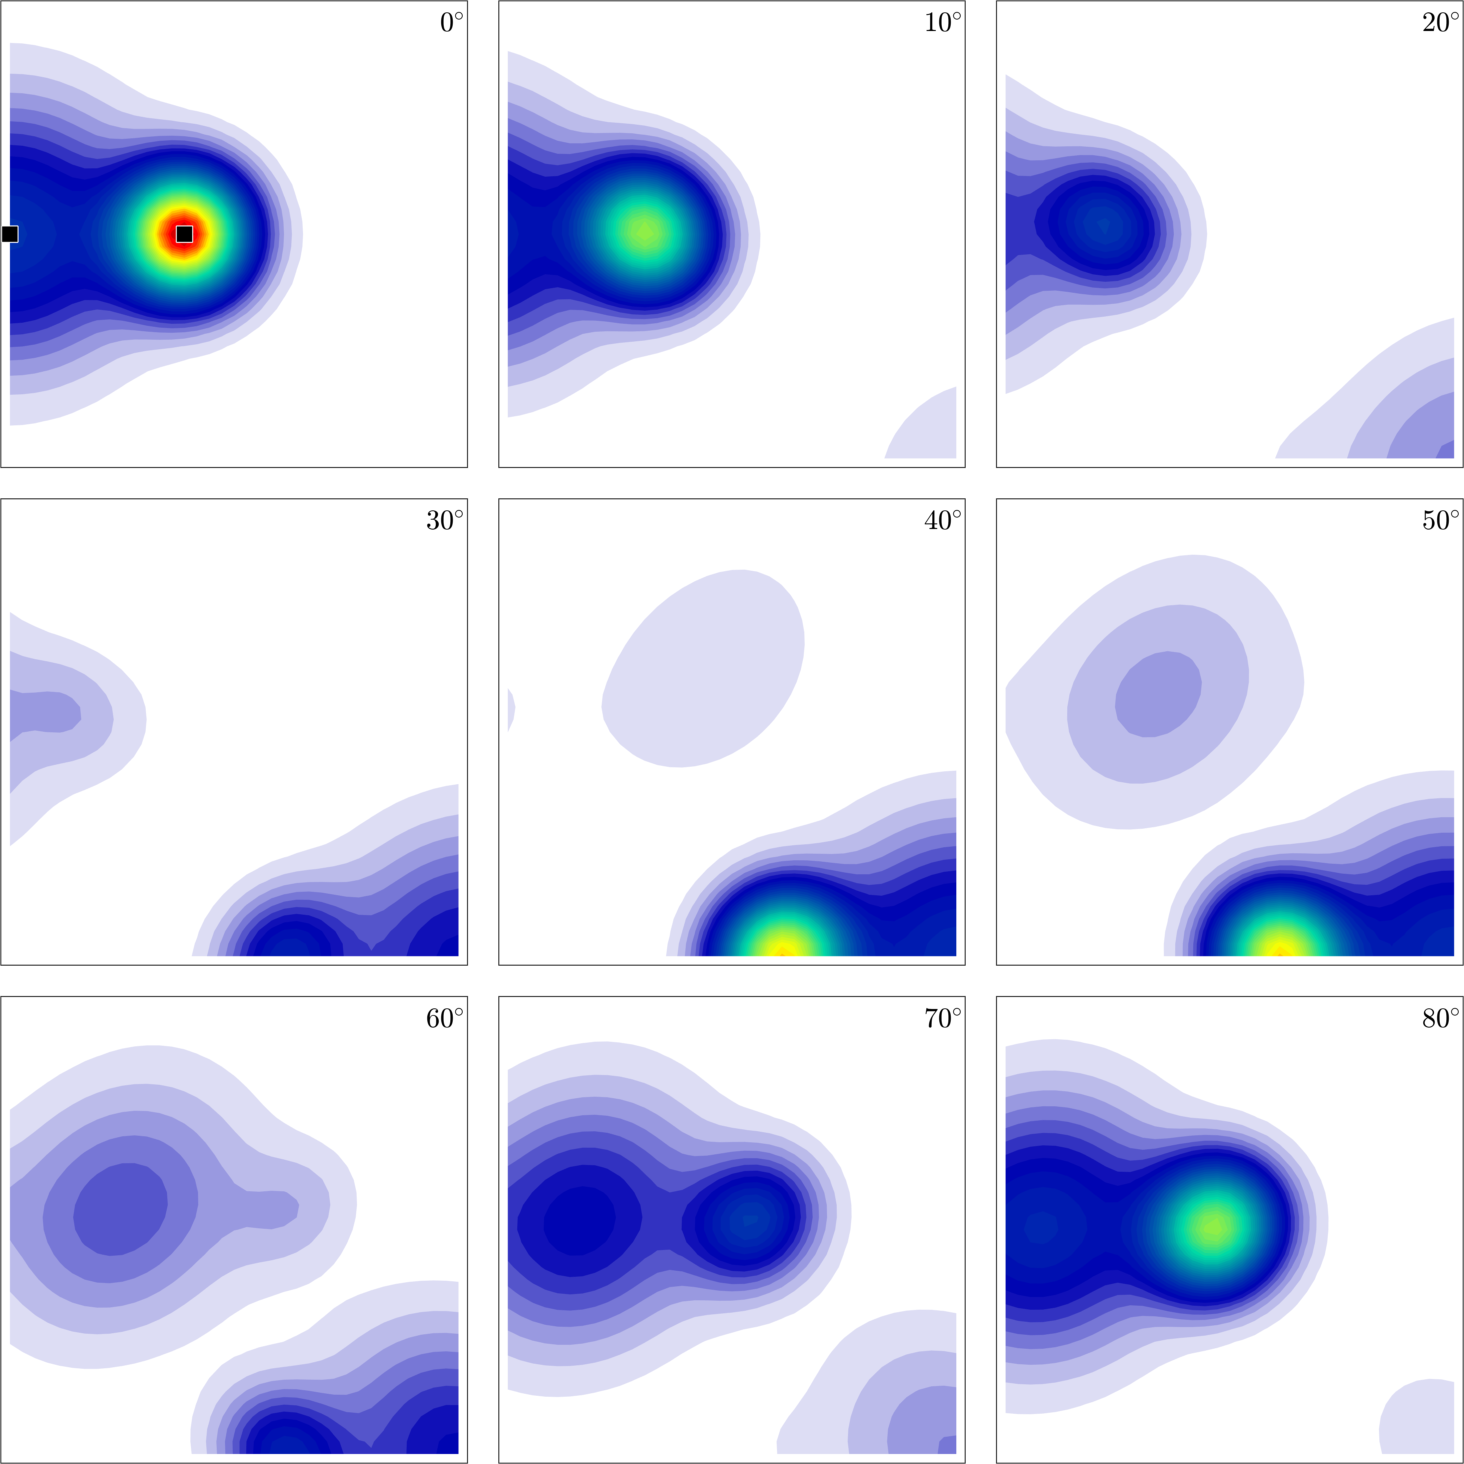
\includegraphics[width=\textwidth]{pic/odfSim1}}%
  \only<2>{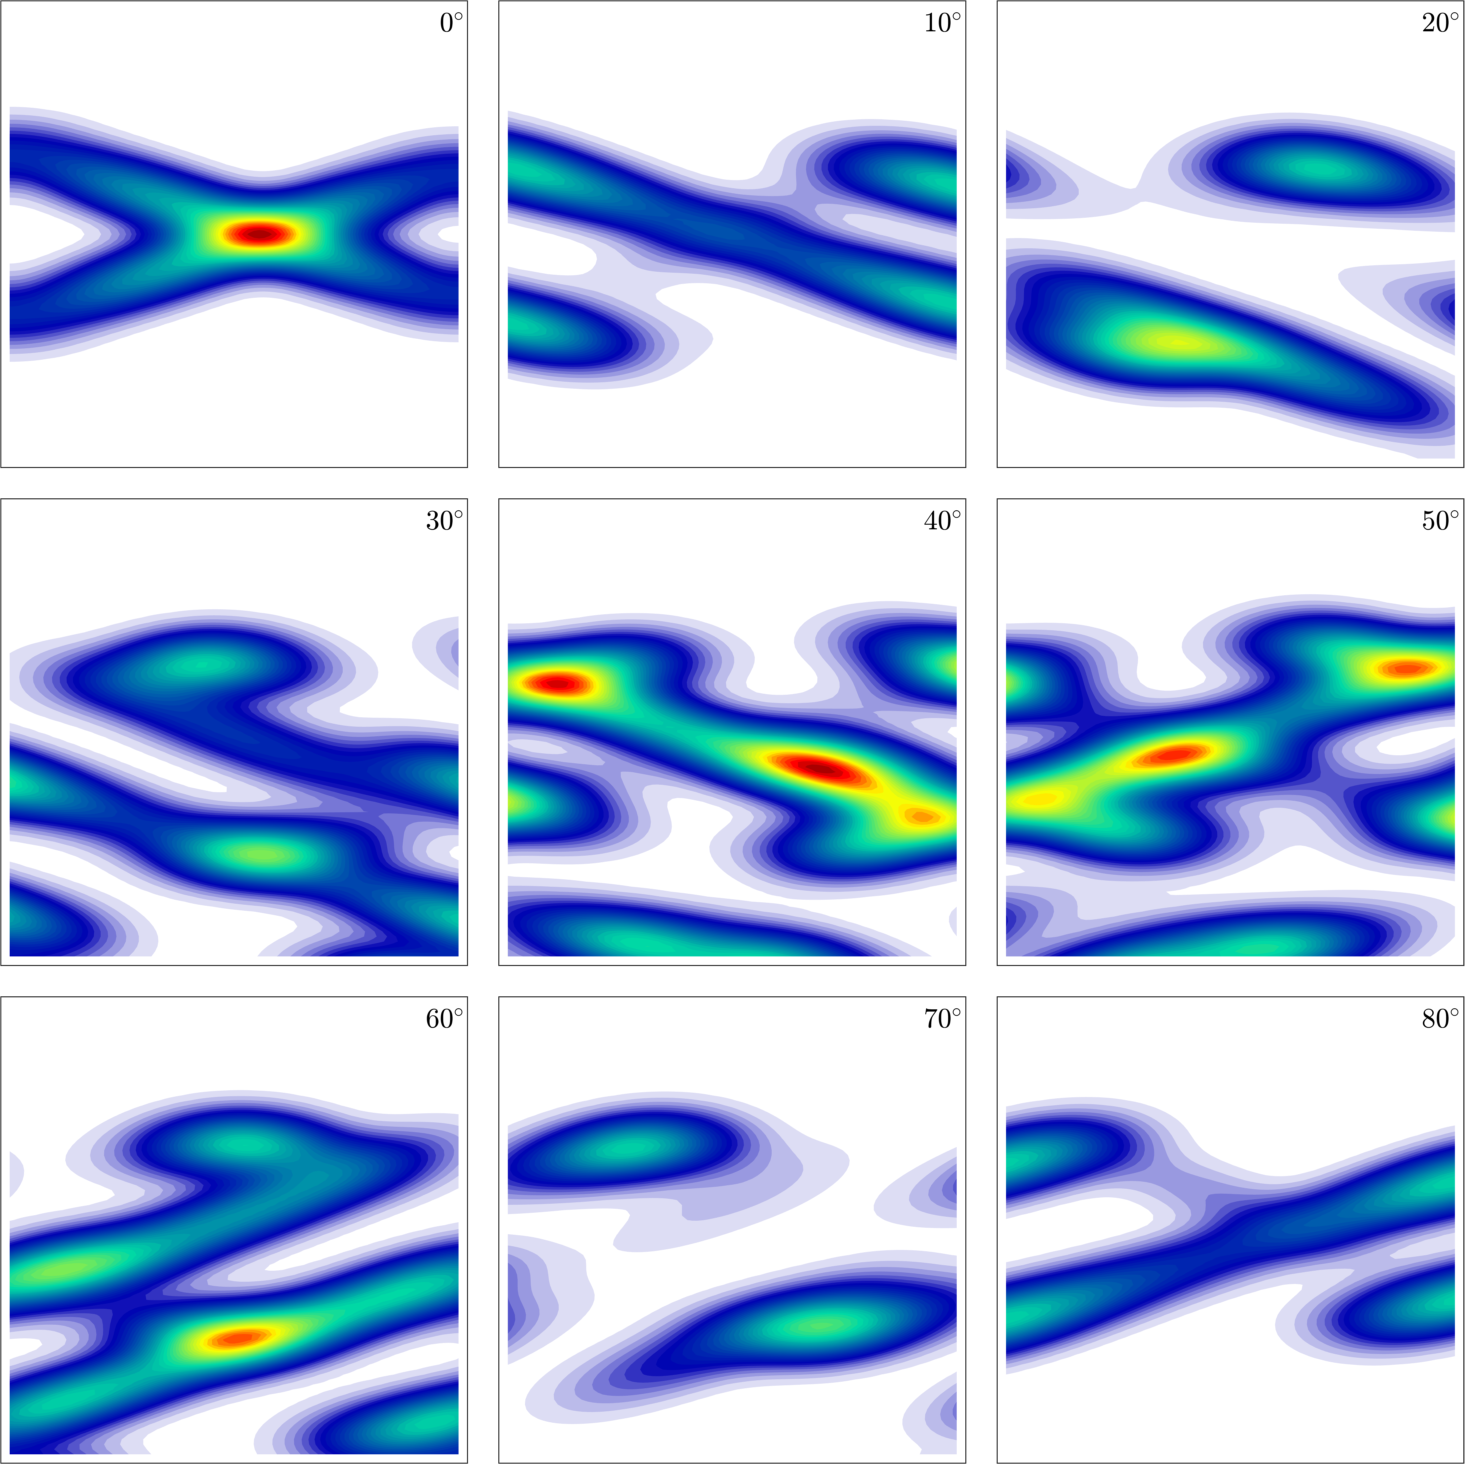
\includegraphics[width=\textwidth]{pic/odfSim2}}
\end{column}
\end{columns}

\end{frame}


\begin{frame}[fragile]
  \frametitle{ODF Sections}

  \begin{columns}

    \begin{column}{0.5\textwidth}

      \begin{lstlisting}[style=input]
plot(odf,'3d')
    \end{lstlisting}

    \pause
    \medskip

      for cubic - orthorhombic symmetry
      Euler angle sections provide a very compact
      visualization of an ODF
      \vspace{-0.2cm}
      \begin{lstlisting}[style=input]
plot(odf,'phi2',(0:10:80)*degree)
    \end{lstlisting}

    \pause
    \medskip

    for triclinic specimen symmetry Euler angle sections are less compact
    \vspace{-0.2cm}
      \begin{lstlisting}[style=input]
plot(odf,'phi2',(0:15:45)*degree)
\end{lstlisting}

    \pause
    \medskip

    for trigonal, tetragonal and hexagon symmetry sigma sections are much more
    compact and easier to interprete \vspace{-0.2cm}
      \begin{lstlisting}[style=input]
plot(odf,'sigma',(0:10:50)*degree)
\end{lstlisting}


    \end{column}
    \begin{column}{0.47\textwidth}

      \only<1>{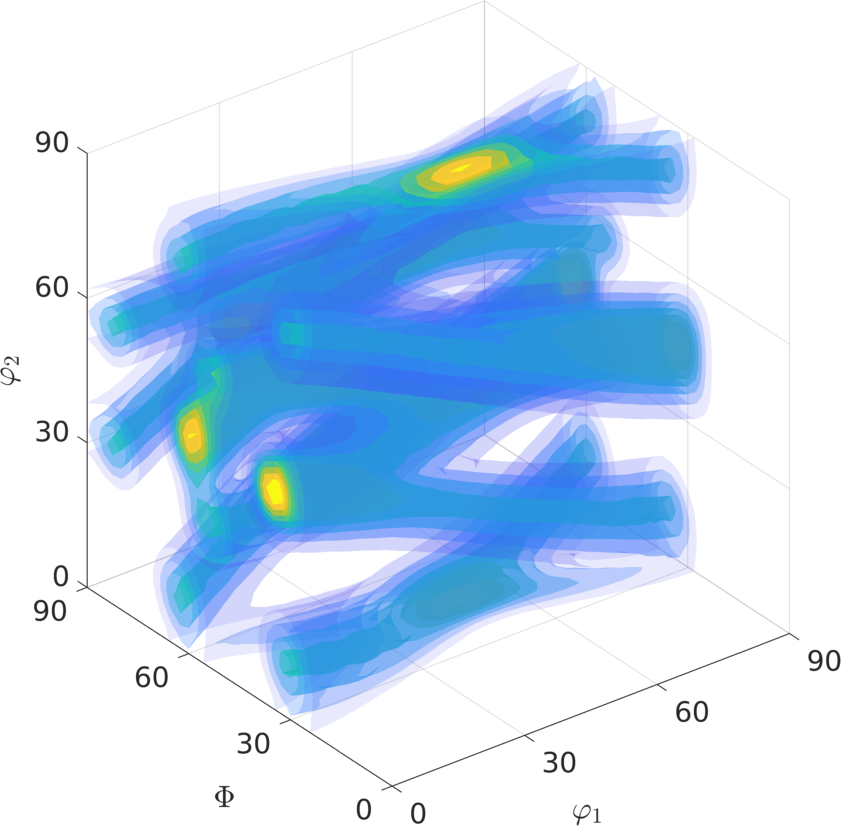
\includegraphics[width=\textwidth]{pic/odfSim2_3d}}
      \only<2>{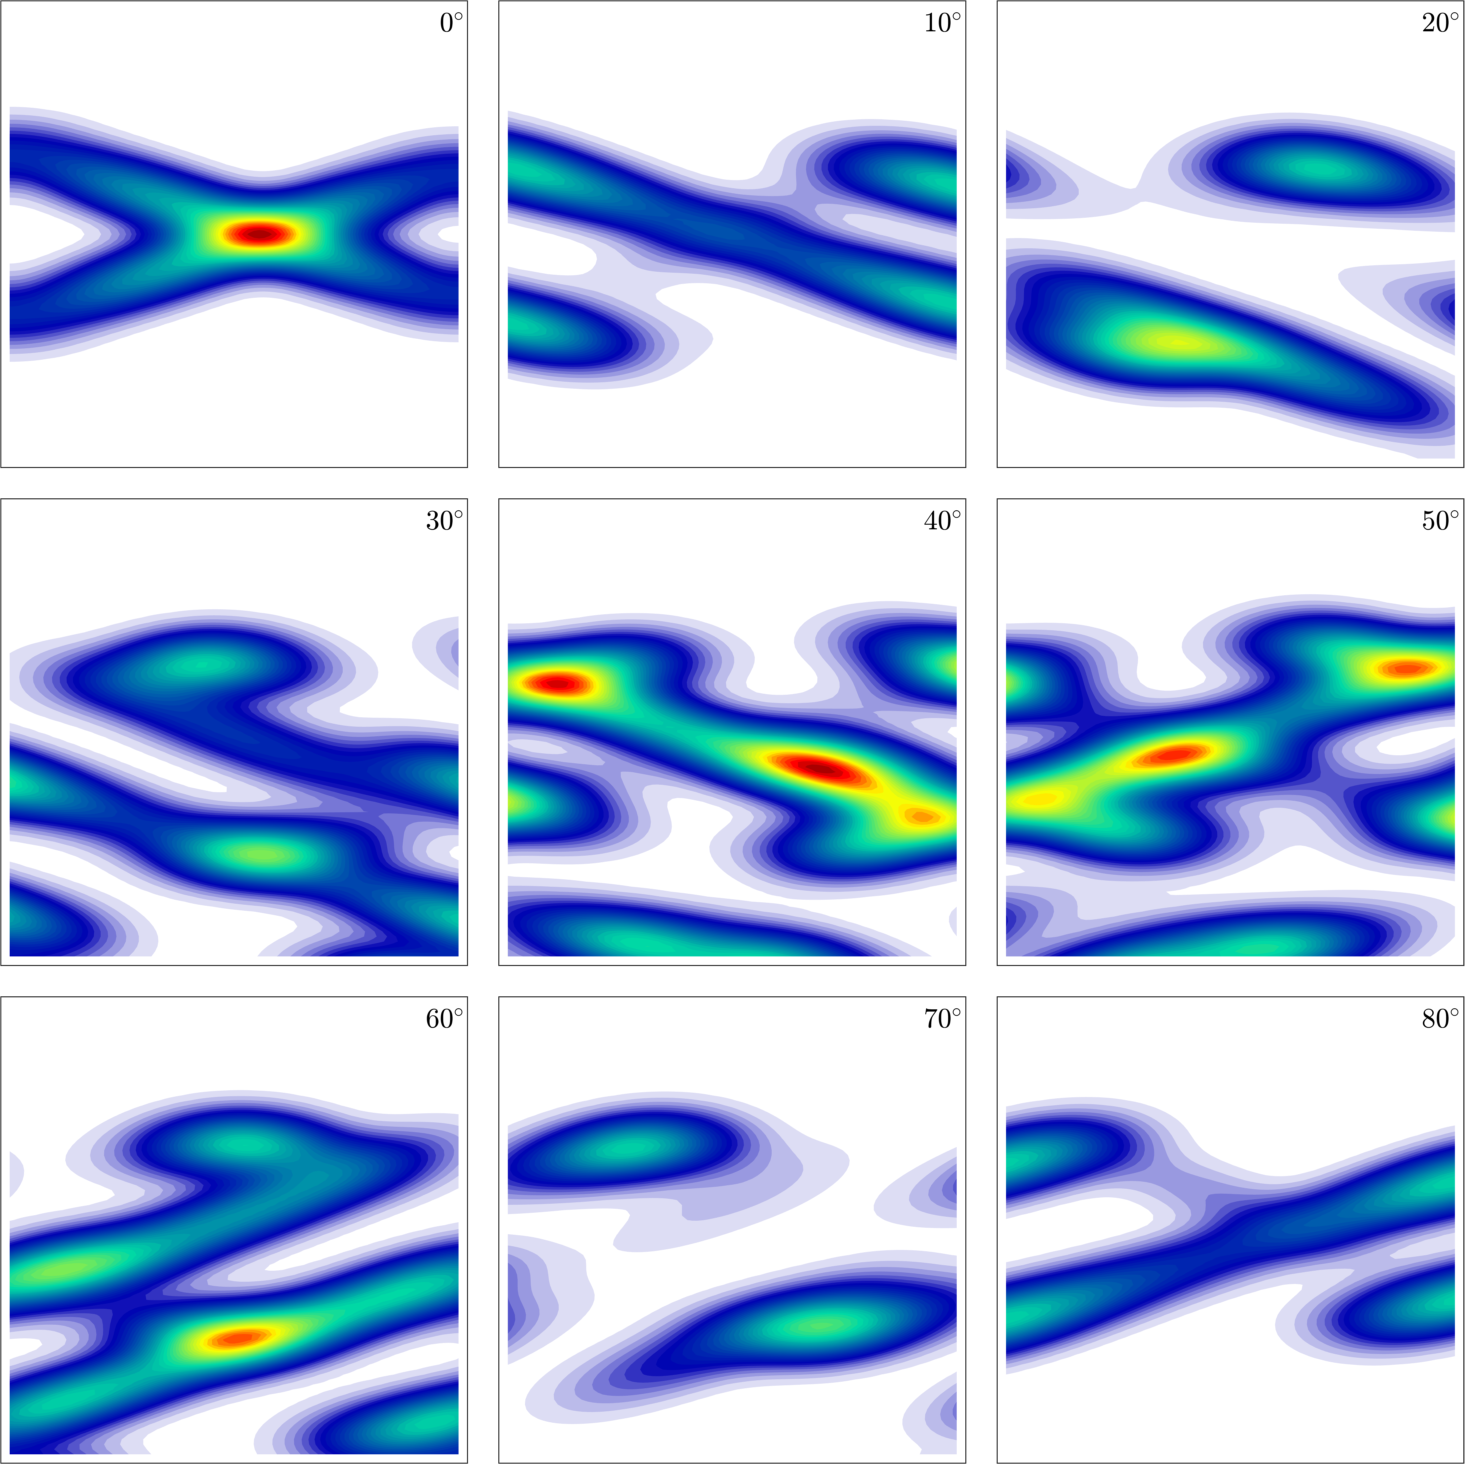
\includegraphics[width=\textwidth]{pic/odfSim2}}
      \only<3>{\vspace{-0.25cm} 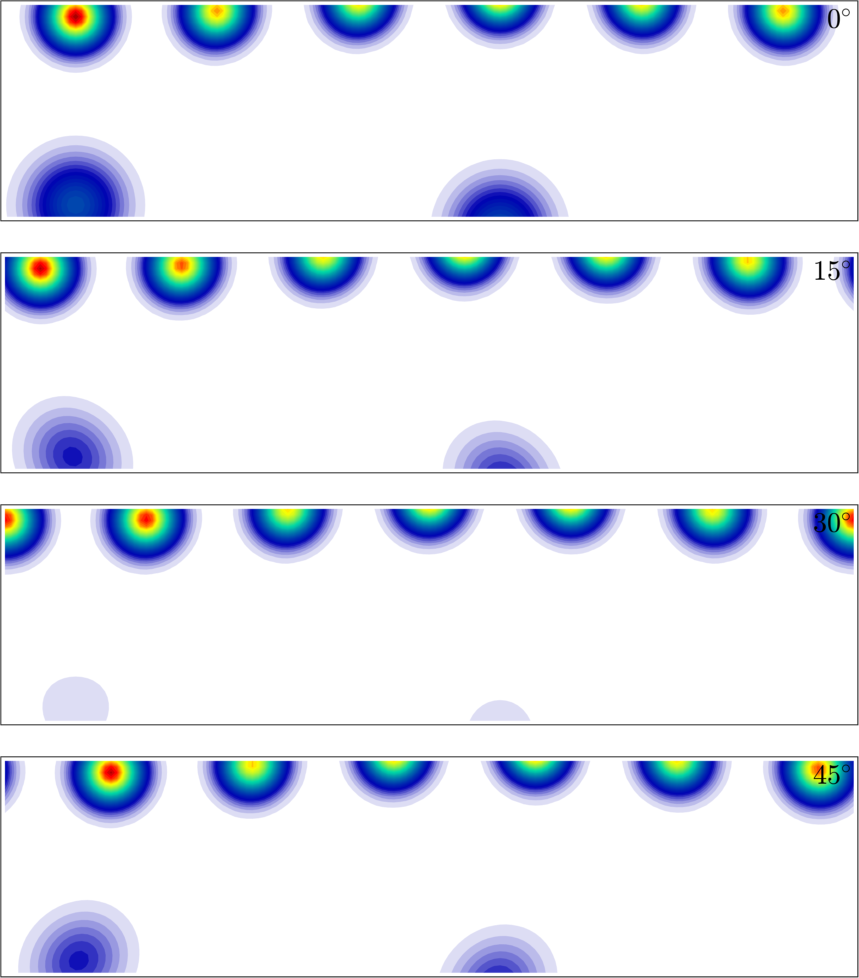
\includegraphics[width=\textwidth]{pic/odfSim3_Euler}}
      \only<4>{\centering
        \vspace{-0.5cm}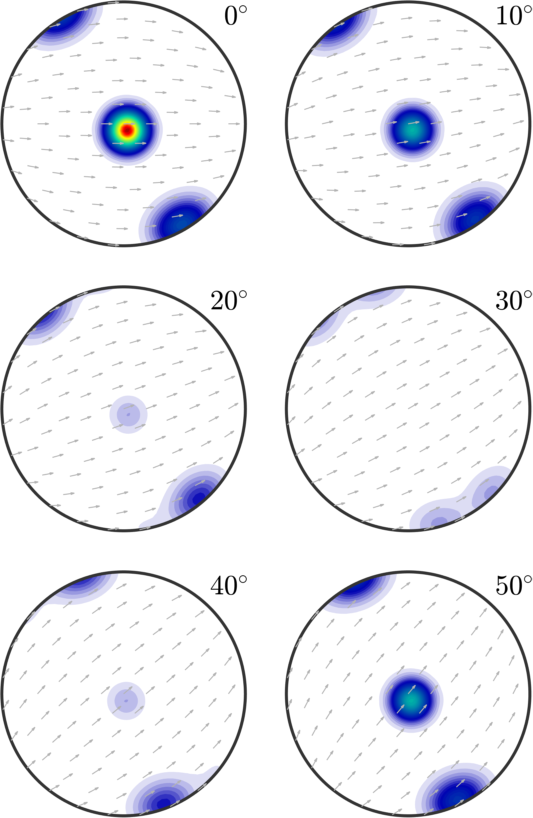
\includegraphics[width=0.75\textwidth]{pic/odfSim3_sigma}
      }

    \end{column}

  \end{columns}


\end{frame}



\begin{frame}[fragile]
  \frametitle{(Inverse) Pole Density Function}

  \begin{columns}

    \begin{column}{0.56\textwidth}

      \begin{lstlisting}[style=input]
h = Miller({0,0,0,1},{2,-1,-1,0},...
          {1,-1,0,0},{2,-1,-1,1},cs)
plotPDF(odf,h)
    \end{lstlisting}

    \pause
    \medskip

    we can compute the pole density function explicitly
    \vspace{-0.2cm}
      \begin{lstlisting}[style=input]
pdf = calcPDF(odf,Miller(0,0,0,1,cs))
    \end{lstlisting}

    \vspace{-0.2cm}
    \begin{lstlisting}[style=output]
pdf = /+S2FunHarmonic+/
 bandwidth: 25
 antipodal: true
    \end{lstlisting}

    \pause
    \medskip

    plotting inverse pole figures
    \vspace{-0.2cm}
    \begin{lstlisting}[style=input]
r=[vector3d.X,vector3d.Y,vector3d.Z]
plotIPDF(odf,r)
      \end{lstlisting}

    \pause
    \medskip

    compute the inverse pole density function
    \vspace{-0.2cm}
      \begin{lstlisting}[style=input]
ipdf = calcIPDF(odf,vector3d.X)
\end{lstlisting}


    \end{column}
    \begin{column}{0.42\textwidth}

      \only<1-2>{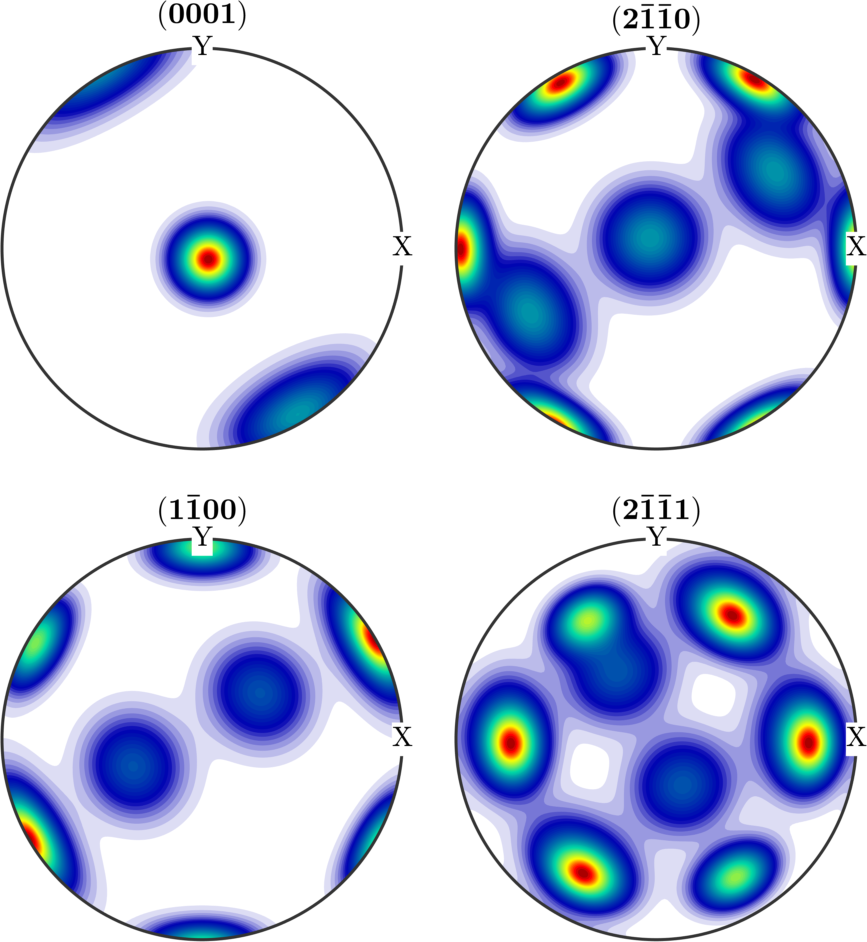
\includegraphics[width=\textwidth]{pic/odfSim3_pf}}
      \only<3-4>{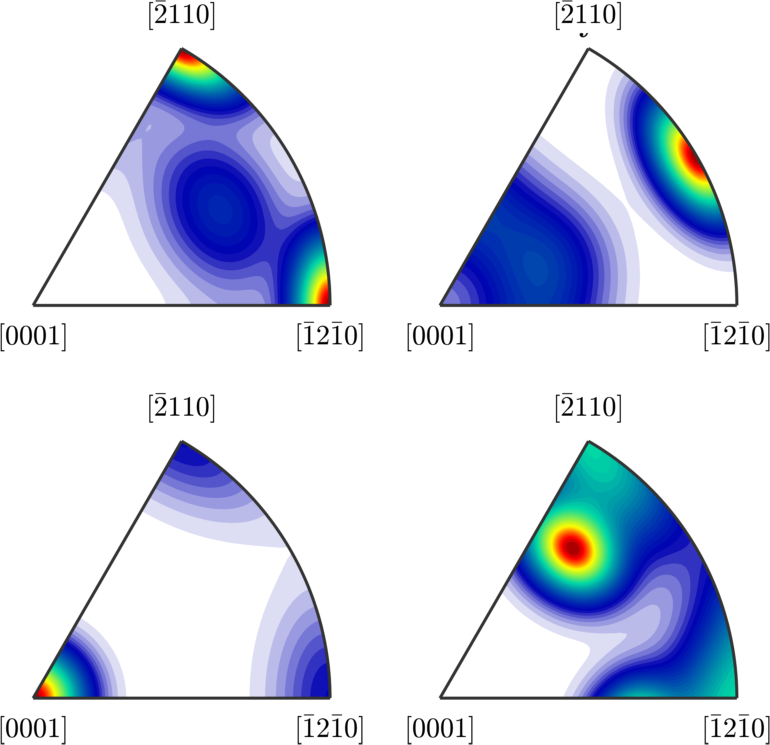
\includegraphics[width=\textwidth]{pic/odfSim3_ipf}}

    \end{column}

  \end{columns}
\end{frame}

\begin{frame}[fragile]
  \frametitle{ODF Characteristics / Texture Strength}

  \vspace{-0.5cm}
  \begin{table}
    \centering

    \begin{tabular}{lllc}
      description
      & formula
      & MTEX command
      & stable\\
      \midrule
      max value
      & $\ds \max_{g} f(g)$
      & \lstinline![value, c] = max(odf)!
      & \textcolor{red!80!black}{\XSolidBrush}
      \\\addlinespace[0.75em]
      texture index
      & $\ds I(f) = \int f(g)^{2} \mathrm d g $
      & \lstinline[style=input]!textureindex(odf)!
      & \textcolor{red!80!black}{\XSolidBrush}\\\addlinespace[0.75em]
      entropy
      & $\ds e = - \int f(g) \ln f(g) dg$
      & \lstinline!entropy(odf)!\\\addlinespace[0.75em]
      ball volume
      & $\ds \int_{\angle(g,c)<r} f(g) \mathrm d g$
      & \lstinline!volume(odf,orientation.Goss(cs),r)!
      & \textcolor{green!80!black}{\CheckmarkBold}\\\addlinespace[0.75em]
      fibre volume
      & $\ds \int_{\angle(g,f)<r} f(g) \mathrm d g$
      & \lstinline!volume(odf,fibre.beta(cs))!
      & \textcolor{green!80!black}{\CheckmarkBold}
      \\\addlinespace[0.75em]
      component volume
      &
      & \lstinline![c, vol] = calcComponents(odf)!
      & \textcolor{green!80!black}{\CheckmarkBold}
    \end{tabular}
  \end{table}

\end{frame}


\begin{frame}
  \frametitle{Spherical Functions - Internal Representation}

  \structure{\texttt{S2FunHarmonic}:} harmonic presentation
  \begin{columns}
    \begin{column}{0.4\textwidth}
      \begin{itemize}
      \item harmonic degree: $\ell$
      \item bandwidth, harmonic cutoff: $L$
      \item harmonic coefficients: $\hat f(\ell,k)$
      \item spherical harmonics: $\Y_{\ell}^{k}$
      \end{itemize}
    \end{column}
    \begin{column}{0.57\textwidth}

      \begin{equation*}
        f(\vec \xi)
        = \sum_{\ell=0}^{L} \sum_{k=-\ell}^{\ell} \hat f(\ell,k) \Y_{\ell}^{k}(\vec
        \xi)
      \end{equation*}
          \end{column}

  \end{columns}

  \pause
  \bigskip

  \structure{\texttt{S2FunTri}:} linear interpolation based on
  \begin{itemize}
  \item nodes: $\vec \eta_{n}$, $n=1,\ldots,N$
  \item values: $f(\vec \eta_{n})$, $n=1,\ldots,N$
  \end{itemize}

  \pause
  \bigskip

  \structure{\texttt{BinghamS2}:} Bingham Distribution
  \begin{columns}
    \begin{column}{0.4\textwidth}
      \begin{itemize}
    \item principal axes: $\vec a_{1}, \vec a_{2}, \vec a_{3}$
    \item principal values: $\kappa_{1}, \kappa_{2}, \kappa_{3}$
    \item normalization constant: $C$
    \end{itemize}
  \end{column}
    \begin{column}{0.57\textwidth}
      \begin{equation*}
        f(\vec \xi) = C \exp\left(\sum_{j=1}^{3} \kappa_{j} \, (\vec \xi \cdot \vec a)^{2}\right)
      \end{equation*}
    \end{column}
    \end{columns}

\end{frame}


\begin{frame}[fragile]
  \frametitle{Defining Spherical Functions}

  \begin{columns}[T,onlytextwidth]

    \begin{column}{0.7\textwidth}
      import directional data from a file
      \vspace{-0.2cm}
  \begin{lstlisting}[style=input]
[v, data] = vector3d.load('smiley.csv',...
      'columnNames',{'x','y','z','value'})
plot(v, data.value);
\end{lstlisting}

\pause
\medskip

linear interpolate \vspace{-0.2cm}
\begin{lstlisting}[style=input]
sF = interp(v, data.value, 'linear')
\end{lstlisting}
\vspace{-0.4cm}
\begin{lstlisting}[style=output]
sF = S2FunTri (show methods, plot)

 vertices: 777 x 1
 values:   777 x 1
\end{lstlisting}

\pause
\medskip

harmonic approximation \vspace{-0.2cm}
\begin{lstlisting}[style=input]
sF = interp(v, data.value, 'harmonic')
\end{lstlisting}
\vspace{-0.4cm}
\begin{lstlisting}[style=output]
sF = S2FunHarmonic (show methods, plot)
 bandwidth: 20
\end{lstlisting}

% %qudrature
% fun = @(v) v.x .* v.y
% sF = S2FunHarmonic.quadrature(fun,'bandwidth',128);
%   \end{lstlisting}
\end{column}
\begin{column}{0.25\textwidth}

  \only<1>{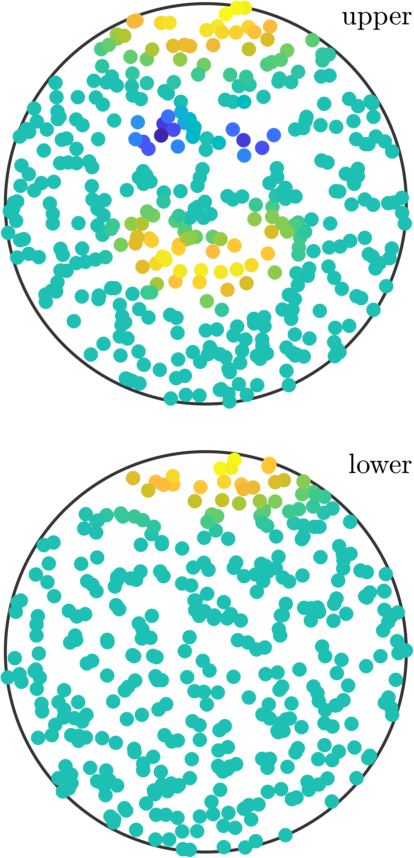
\includegraphics[width=\textwidth]{pic/vecData}}
  \only<2>{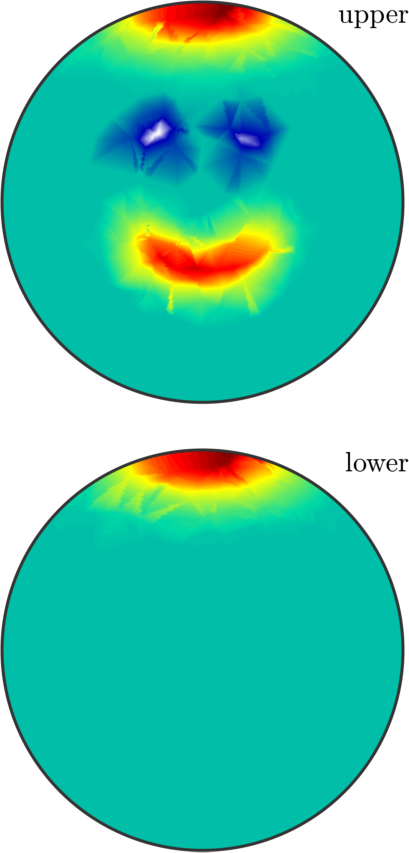
\includegraphics[width=\textwidth]{pic/vecDataLin}}
  \only<3>{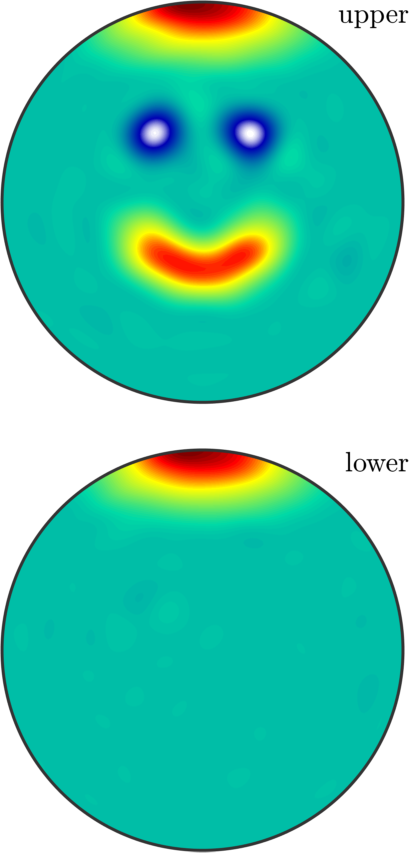
\includegraphics[width=\textwidth]{pic/vecDataHarm}}

\end{column}
\end{columns}



\end{frame}

\begin{frame}[fragile]
  \frametitle{Orientation Distribution Functions - Internal Representation}

  \structure{\texttt{SO3FunHarmonic, FourierODF}:} harmonic presentation
  \begin{columns}
    \begin{column}{0.4\textwidth}
      \begin{itemize}
      \item harmonic degree: $\ell$
      \item bandwidth, harmonic cutoff: $L$
      \item harmonic coefficients: $\hat f(\ell,k,k')$
      \item Wigner D functions: $D_{\ell}^{k,k'}$
      \end{itemize}
    \end{column}
    \begin{column}{0.57\textwidth}

      \begin{equation*}
        f(\mathtt{ori})
        = \sum_{\ell=0}^{L} \sum_{k,k'=-\ell}^{\ell} \hat f(\ell,k,k') D_{\ell}^{k,k}(\mathtt{ori})
      \end{equation*}
    \end{column}

  \end{columns}

  \pause
  \bigskip

  \structure{\texttt{SO3FunHandle}:} explicit orientation dependent function
  \begin{lstlisting}[style=input]
fun = @(ori) angle(ori)
SO3F = SO3FunHandle(fun)
  \end{lstlisting}

  \pause
  \bigskip

  \structure{\texttt{SO3FunBingham, BinghamODF}:} Bingham Distribution
  \begin{columns}
    \begin{column}{0.4\textwidth}
      \begin{itemize}
    \item principal axes: $\mathtt{ori}_{1},\ldots,\mathtt{ori}_{4}$
    \item principal values: $\kappa_{1}, \kappa_{2}, \kappa_{3}, \kappa_{4}$
    \item normalization constant: $C$
    \end{itemize}
  \end{column}
    \begin{column}{0.57\textwidth}
      \begin{equation*}
        f(\mathtt{ori}) = C \exp\left(\sum_{j=1}^{4} \kappa_{j} \, (\mathtt{ori} \cdot \mathtt{ori}_{j})^{2}\right)
      \end{equation*}
    \end{column}
    \end{columns}

  \end{frame}

\begin{frame}
  \frametitle{Orientation Distribution Functions}

  \structure{\texttt{SO3FunRBF, UnimodalODF}:} superposition of unimodal components
  \begin{columns}
    \begin{column}{0.4\textwidth}
      \begin{itemize}
      \item center orientations: $\mathtt{ori}_{n}$
      \item weights: $c_{n}$
      \item kernel function: $\psi$
      \end{itemize}
    \end{column}
    \begin{column}{0.57\textwidth}

      \begin{equation*}
        f(\mathtt{ori})
        = \sum_{n=1}^{N} c_{n} \psi(\omega(\mathtt{ori}, \mathtt{ori}_{n}))
      \end{equation*}
          \end{column}

  \end{columns}

  \pause
  \bigskip

  \structure{\texttt{SO3FunCBF, fibreODF}:} superposition of fiber symmetric components
    \begin{columns}
    \begin{column}{0.4\textwidth}
      \begin{itemize}
      \item fibers: $\mathtt{f}_{n}$
      \item weights: $c_{n}$
      \item kernel function: $\psi$
      \end{itemize}
    \end{column}
    \begin{column}{0.57\textwidth}

      \begin{equation*}
        f(\mathtt{ori})
        = \sum_{n=1}^{N} c_{n} \psi(\omega(\mathtt{ori}, \mathtt{f}_{n}))
      \end{equation*}
    \end{column}

  \end{columns}

  \pause
  \bigskip

  \structure{\texttt{uniformODF}:} constant ODF
  \begin{columns}
    \begin{column}{0.4\textwidth}
      \begin{itemize}
      \item constant: $C$
    \end{itemize}
  \end{column}
    \begin{column}{0.57\textwidth}
      \begin{equation*}
        f(\mathtt{ori}) = C
      \end{equation*}
    \end{column}
  \end{columns}

\end{frame}


\begin{frame}
  \frametitle{Approximation, Interpolation and Quadrature}
  
\end{frame}


\end{document}
